\documentclass[letterpaper]{article}
\usepackage{geometry}
\usepackage{dirtree}
\usepackage{listings}
\usepackage{relsize}
\usepackage{graphicx}
\usepackage{float}

\graphicspath{ {./images/} }

\lstset{basicstyle=\footnotesize\ttfamily}
\geometry{left=20mm, right=20mm}
\newcommand{\Cpp}{\mbox{C\kern-.1em\raisebox{.35ex}{\smaller{\smaller{+\kern-0.05em+}}}}}

\begin{document}
\title{Multi-Directory Projects in Qt with CMake}
\author{Jeffrey K. Bienstadt}
\date{10 February, 2004}
\maketitle

\begin{abstract}
  The Qt framework and the Qt~Creator IDE support projects that are split across
  multiple directories. Unfortunately, the IDE does not provide mechanisms for
  managing such projects. This article will address this and demonstrate how to
  create and manage multi-directory projects with Qt.
\end{abstract}

Write something introductory here.

This article assumes some previous exposure to Qt, both the framework itself and
the Qt~Creator integrated development environment (IDE). We will be using version
6.6.1 of the Qt framework, and Qt~Creator version 12.0.2.

We will create a multi-directory project with a main application and a helpful
library with a directory structure like this:
\begin{figure}[h!]
\centering
\begin{minipage}{5cm}
  \dirtree{%
  .1 App.
  .2 OurApp.
  .2 OurLib.
}
\end{minipage}
\end{figure}

The main application will be in the directory \verb|App/OurApp|, and the supporting
library will be in the directory \verb|App/OurLib|.

We will start by creating a directory named \verb|App| to contain our application.
Create this directory wherever you like.

Next we will use Qt~Creator to generate our main application project and our
library project, both within the new \verb|App| directory. We will start with the main application. Using Qt~Creator,
create a new project, either from the \textbf{File} menu
(\textbf{New Project\ldots}) or by selecting \textbf{Create Project\ldots}
from the \textbf{Welcome} page. In the \textbf{New Project} dialog, select 
\textbf{Application (Qt)} in the left-most pane, and \textbf{Qt Widgets Application}
in the center pane, as shown in Figure~\ref{fig:create_ourapp_1}, then press the \textbf{Choose\ldots} button.
\begin{figure}[H]
  \centering
  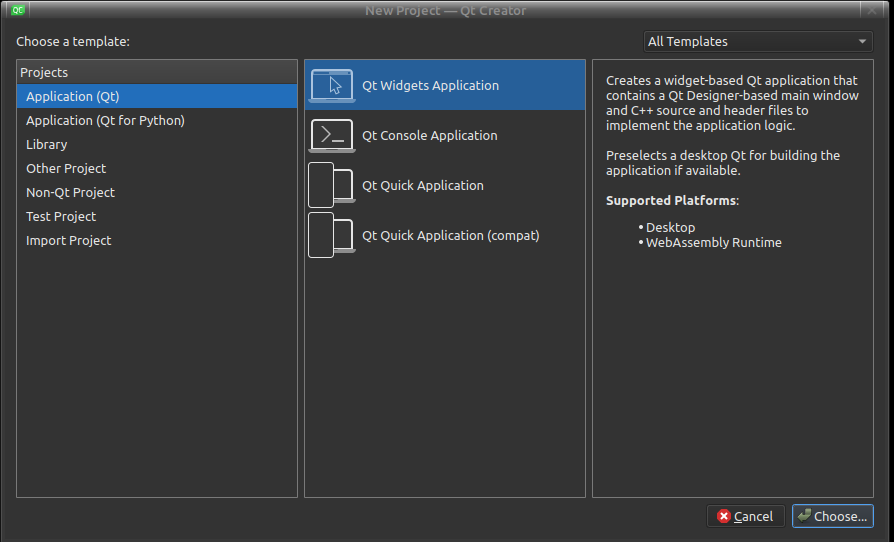
\includegraphics[width=0.7\textwidth]{create_ourapp_1.png}
  \caption{Create the OurApp application.}
  \label{fig:create_ourapp_1}
\end{figure}

On the \textbf{Project Location} dialog, name the project \textbf{OurApp},
and create the project in the newly-created \textbf{App} directory, as shown
in Figure~\ref{fig:create_ourapp_2}, then
click the \textbf{Next} button.
\begin{figure}[H]
  \centering
  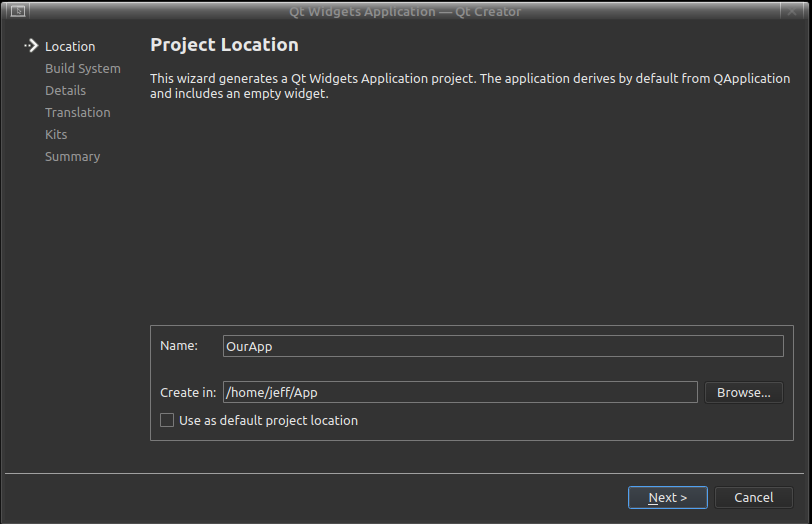
\includegraphics[width=0.7\textwidth]{create_ourapp_2.png}
  \caption{Name and location of the OurApp application.}
  \label{fig:create_ourapp_2}
\end{figure}

On the \textbf{Define Build System} dialog, shown in Figure~\ref{fig:create_ourapp_3},
select \textbf{CMake} as the build system, and click \textbf{Next}.
\begin{figure}[H]
  \centering
  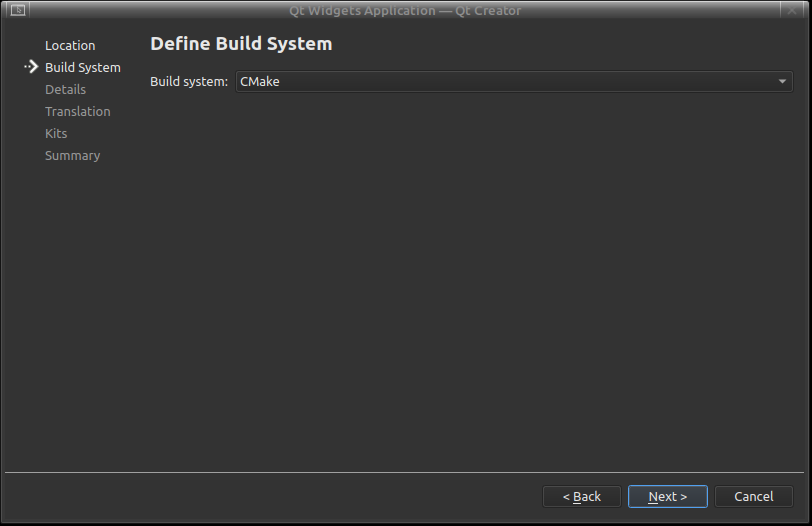
\includegraphics[width=0.7\textwidth]{create_ourapp_3.png}
  \caption{Select CMake as the build system.}
  \label{fig:create_ourapp_3}
\end{figure}

On the \textbf{Class Information} dialog you can just leave the default values
for everything and click the \textbf{Next} button (Figure~\ref{fig:create_ourapp_4}).
\begin{figure}[H]
  \centering
  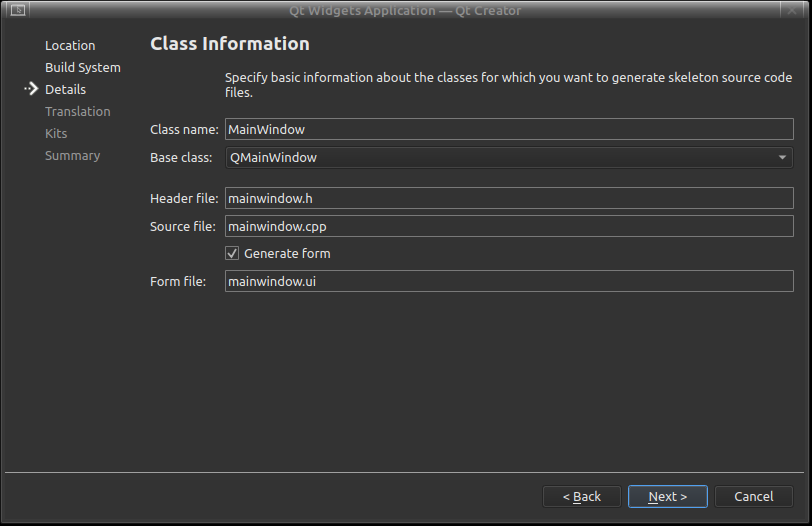
\includegraphics[width=0.7\textwidth]{create_ourapp_4.png}
  \caption{Class Information dialog.}
  \label{fig:create_ourapp_4}
\end{figure}

Click \textbf{Next} on the \textbf{Translation File} dialog (Figure~\ref{fig:create_ourapp_5}),
leaving the default values.
\begin{figure}[H]
  \centering
  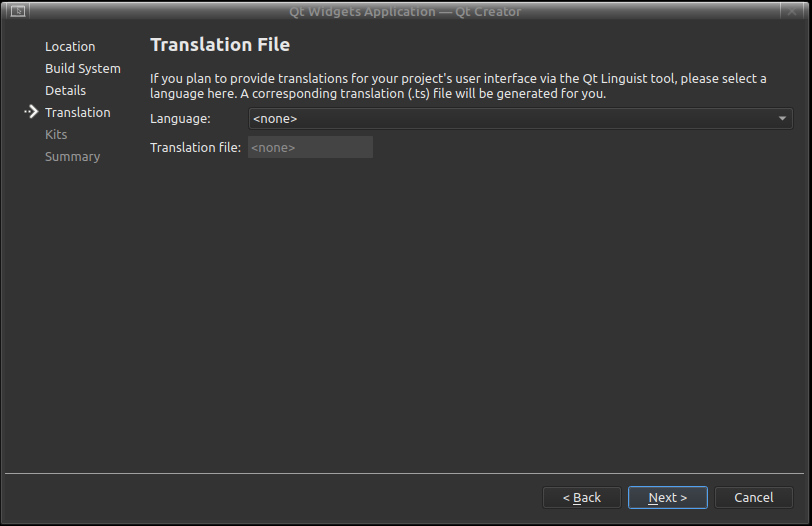
\includegraphics[width=0.7\textwidth]{create_ourapp_5.png}
  \caption{Translation File dialog.}
  \label{fig:create_ourapp_5}
\end{figure}


On the \textbf{Kit Selection} dialog, select a \textbf{Desktop} kit as shown
in Figure~\ref{fig:create_ourapp_6} and click the \textbf{Next} button.
\begin{figure}[H]
  \centering
  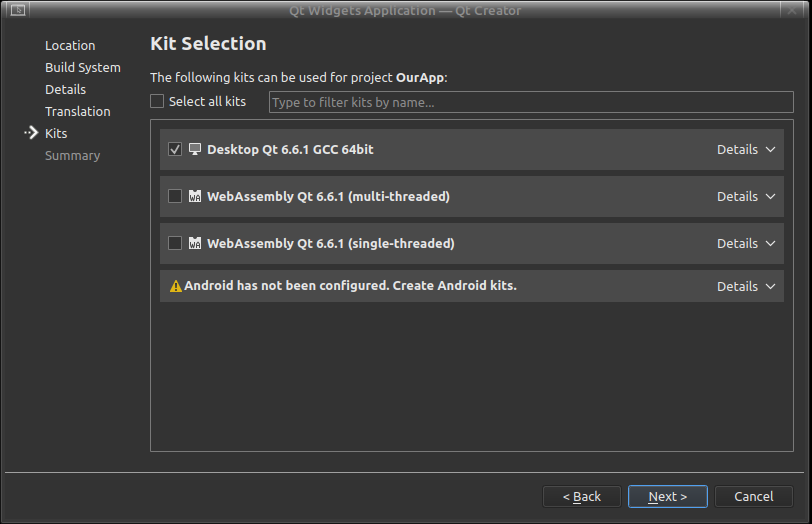
\includegraphics[width=0.7\textwidth]{create_ourapp_6.png}
  \caption{Select a Desktop kit.}
  \label{fig:create_ourapp_6}
\end{figure}

Finally, on the \textbf{Project Management} dialog (Figure~\ref{fig:create_ourapp_7}), leave the default values
and click the \textbf{Finish} button. Qt~Creator will generate a GUI project
in the \verb|App/OurApp| directory.
\begin{figure}[H]
  \centering
  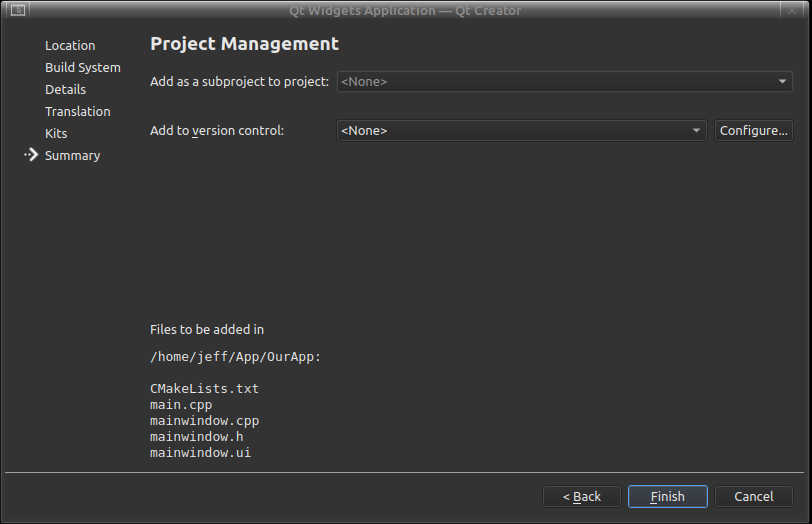
\includegraphics[width=0.7\textwidth]{create_ourapp_7.png}
  \caption{Project Management dialog.}
  \label{fig:create_ourapp_7}
\end{figure}

This project contains a \verb|CMakeLists.txt| file with the following content:
\begin{lstlisting}
  cmake_minimum_required(VERSION 3.5)

  project(OurApp VERSION 0.1 LANGUAGES CXX)
  
  set(CMAKE_AUTOUIC ON)
  set(CMAKE_AUTOMOC ON)
  set(CMAKE_AUTORCC ON)
  
  set(CMAKE_CXX_STANDARD 17)
  set(CMAKE_CXX_STANDARD_REQUIRED ON)
  
  find_package(QT NAMES Qt6 Qt5 REQUIRED COMPONENTS Widgets)
  find_package(Qt${QT_VERSION_MAJOR} REQUIRED COMPONENTS Widgets)
  
  set(PROJECT_SOURCES
          main.cpp
          mainwindow.cpp
          mainwindow.h
          mainwindow.ui
  )
  
  if(${QT_VERSION_MAJOR} GREATER_EQUAL 6)
      qt_add_executable(OurApp
          MANUAL_FINALIZATION
          ${PROJECT_SOURCES}
      )
  # Define target properties for Android with Qt 6 as:
  #    set_property(TARGET OurApp APPEND PROPERTY QT_ANDROID_PACKAGE_SOURCE_DIR
  #                 ${CMAKE_CURRENT_SOURCE_DIR}/android)
  # For more information, see https://doc.qt.io/qt-6/qt-add-executable.html#target-creation
  else()
      if(ANDROID)
          add_library(OurApp SHARED
              ${PROJECT_SOURCES}
          )
  # Define properties for Android with Qt 5 after find_package() calls as:
  #    set(ANDROID_PACKAGE_SOURCE_DIR "${CMAKE_CURRENT_SOURCE_DIR}/android")
      else()
          add_executable(OurApp
              ${PROJECT_SOURCES}
          )
      endif()
  endif()
  
  target_link_libraries(OurApp PRIVATE Qt${QT_VERSION_MAJOR}::Widgets)
  
  # Qt for iOS sets MACOSX_BUNDLE_GUI_IDENTIFIER automatically since Qt 6.1.
  # If you are developing for iOS or macOS you should consider setting an
  # explicit, fixed bundle identifier manually though.
  if(${QT_VERSION} VERSION_LESS 6.1.0)
    set(BUNDLE_ID_OPTION MACOSX_BUNDLE_GUI_IDENTIFIER com.example.OurApp)
  endif()
  set_target_properties(OurApp PROPERTIES
      ${BUNDLE_ID_OPTION}
      MACOSX_BUNDLE_BUNDLE_VERSION ${PROJECT_VERSION}
      MACOSX_BUNDLE_SHORT_VERSION_STRING ${PROJECT_VERSION_MAJOR}.${PROJECT_VERSION_MINOR}
      MACOSX_BUNDLE TRUE
      WIN32_EXECUTABLE TRUE
  )
  
  include(GNUInstallDirs)
  install(TARGETS OurApp
      BUNDLE DESTINATION .
      LIBRARY DESTINATION ${CMAKE_INSTALL_LIBDIR}
      RUNTIME DESTINATION ${CMAKE_INSTALL_BINDIR}
  )
  
  if(QT_VERSION_MAJOR EQUAL 6)
      qt_finalize_executable(OurApp)
  endif()
  \end{lstlisting}

  Now that we have our main application, we can augment it with a custom library.
  Create a new project, this time select \textbf{Library} in the left-most pane
  and \textbf{\Cpp~Library} in the center pane, as shown in Figure~\ref{fig:create_ourlib_1},
  and click the \textbf{Choose\ldots} button.
  \begin{figure}[H]
    \centering
    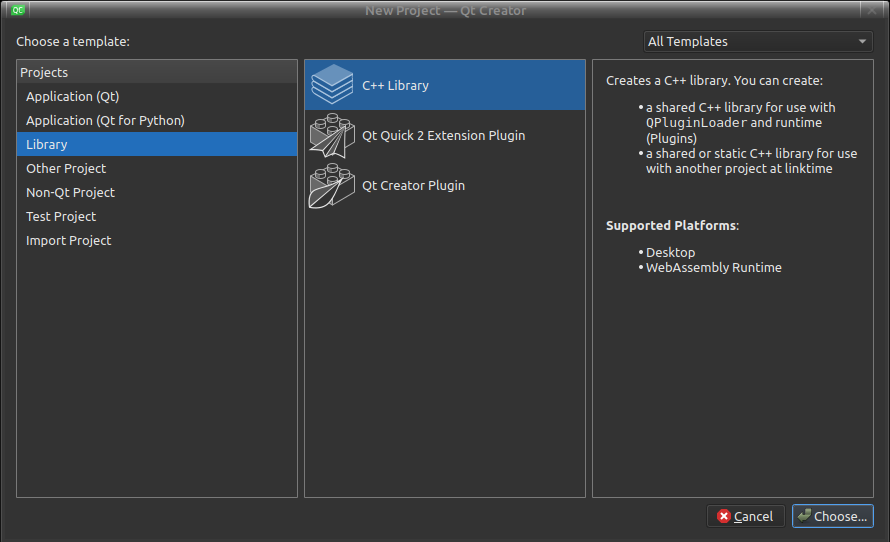
\includegraphics[width=0.7\textwidth]{create_ourlib_1.png}
    \caption{Create the \Cpp\ library dialog.}
    \label{fig:create_ourlib_1}
  \end{figure}
  
  On the Project Location dialog (Figure~\ref{fig:create_ourlib_2}), name the project \textbf{OurLib} and create the project within the
  \textbf{App} directory along side the \textbf{OurApp} project directory. 
  \begin{figure}[H]
    \centering
    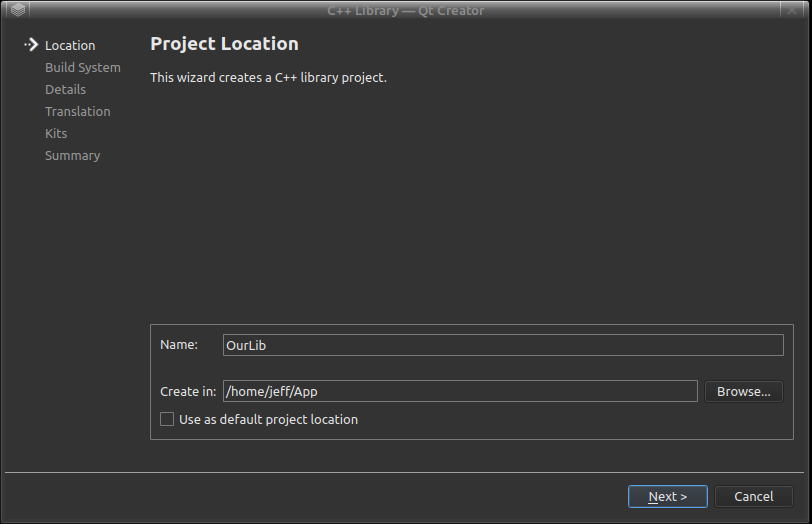
\includegraphics[width=0.7\textwidth]{create_ourlib_2.png}
    \caption{Provide the name and location of the library.}
    \label{fig:create_ourlib_2}
  \end{figure}

  As before, in the \textbf{Define Build System} dialog
  choose \textbf{CMake} as the build system and click \textbf{Next}.

  On the \textbf{Define Project Details} dialog, select \textbf{Statically Linked Library}
  as the type, and select \textbf{Widgets} as the Qt~module (Figure~\ref{fig:create_ourlib_4}).
  Leave the rest to their default values and click \textbf{Next}.
  \begin{figure}[H]
    \centering
    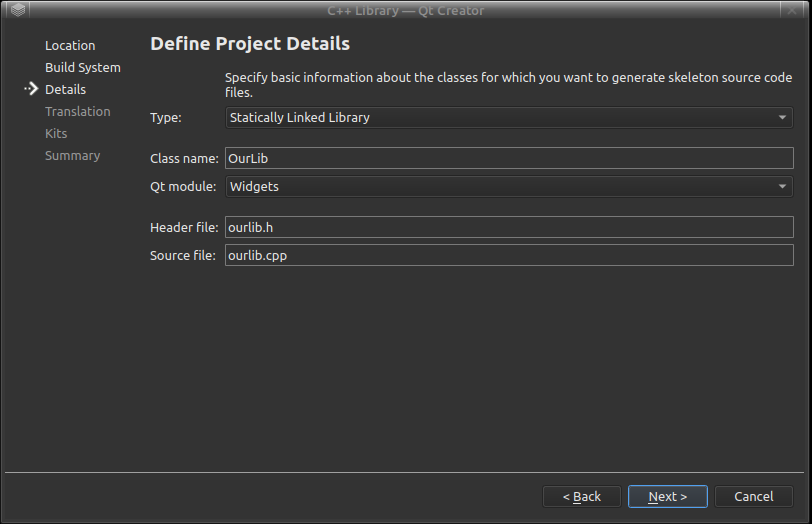
\includegraphics[width=0.7\textwidth]{create_ourlib_4.png}
    \caption{Provide the library type and the required Qt module.}
    \label{fig:create_ourlib_4}
  \end{figure}

  As we did before, click \textbf{Next} to leave the \textbf{Translation File} values to
  their defaults, and select a \textbf{Desktop} kit on the \textbf{Kit Selection} dialog
  and click \textbf{Next}. Again, leave the \textbf{Project Management} dialog to itself
  default values and click \textbf{Finish} to generate the library project.

  Among the files in the library project is a \verb|CMakeLists.txt| file. This one is a bit
  simpler than the one for the \verb|OurApp| project:
  \begin{lstlisting}
    cmake_minimum_required(VERSION 3.14)

    project(OurLib LANGUAGES CXX)
    
    set(CMAKE_AUTOUIC ON)
    set(CMAKE_AUTOMOC ON)
    set(CMAKE_AUTORCC ON)
    set(CMAKE_CXX_STANDARD 17)
    set(CMAKE_CXX_STANDARD_REQUIRED ON)
    
    find_package(QT NAMES Qt6 Qt5 REQUIRED COMPONENTS Widgets)
    find_package(Qt${QT_VERSION_MAJOR} REQUIRED COMPONENTS Widgets)
    
    add_library(OurLib STATIC
      ourlib.cpp
      ourlib.h
    )
    
    target_link_libraries(OurLib PRIVATE Qt${QT_VERSION_MAJOR}::Widgets)
    
    target_compile_definitions(OurLib PRIVATE OURLIB_LIBRARY)    
  \end{lstlisting}


  We now have two separate projects, an application and a library, as shown in Figure~\ref{fig:init_layout}.

  \begin{figure}[H]
    \centering
    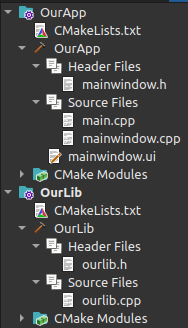
\includegraphics{initial_project_layout.png}
    \caption{Layout for two projects.}
    \label{fig:init_layout}
  \end{figure}

  However, they are just that, two separate projects that have no real connection.
  We can build each project, but they have nothing to do with each other. We need
  to make sure that Qt~Creator knows that the application OurApp requires the static
  library OurLib.

  Before we go any further, let's modify the library's code so that it does something
  useful for the application. The library header file \verb|outlib.h| contains a
  simple class definition:
  \begin{lstlisting}
#ifndef OURLIB_H
#define OURLIB_H

class OurLib
{
public:
    OurLib();
};

#endif // OURLIB_H
  \end{lstlisting}
  The library souce file \verb|ourlib.cpp| contains just an empty definition of the class' constructor:
  \begin{lstlisting}
#include "ourlib.h"

OurLib::OurLib() {}
  \end{lstlisting}

  Let's get rid of the class and provide a simple free function that greets the user.
  Our new \verb|ourlib.h| looks like
\begin{lstlisting}
#ifndef OURLIB_H
#define OURLIB_H

#include <QWidget>

void sayHello(QWidget *parent);

#endif // OURLIB_H
  \end{lstlisting}
  while our new \verb|ourlib.cpp| file defines the \verb|sayHello| function:
  \begin{lstlisting}
  #include "ourlib.h"

  #include <QMessageBox>

void sayHello(QWidget *parent)
{
    QMessageBox::information(parent, "Hello", "Hello from OurLib!");
}
  \end{lstlisting}

  The Qt-generated \verb|main.cpp| file in the OurApp application is very simple:
  \begin{lstlisting}
#include "mainwindow.h"

#include <QApplication>

int main(int argc, char *argv[])
{
    QApplication a(argc, argv);
    MainWindow w;
    w.show();
    return a.exec();
}
  \end{lstlisting}

  We will modify this file to make use of our library by adding two lines of code:
  \begin{lstlisting}
#include "mainwindow.h"
#include "../OurLib/ourlib.h"

#include <QApplication>

int main(int argc, char *argv[])
{
    QApplication a(argc, argv);
    MainWindow w;
    w.show();
    sayHello(&w);
    return a.exec();
}
  \end{lstlisting}

  Here we added the \verb|#include| directive to bring in our library's header file from the \verb|OurLib|
  project directory, and added a call to the \verb|sayHello| function provided by the library.
  When we build our projects, the \verb|OurLib| project compiles and links, producing a library file.
  However, the \verb|OurApp| project compiles but fails to link, with an error saying that there
  is an undefined reference to the \verb|sayHello| function. This is because the \verb|OurApp| project
  knows nothing about the \verb|OurLib| library and isn't linking to it.

  It's time to change our project model a bit. We currently have two separate projects,
  each with its own ``top-level'' \verb|CMakeLists.txt| file. We are going to change this
  so that there is a single top-level \verb|CMakeLists.txt| file, and slightly modified
  \verb|CMakeLists.txt| files in each of the project directories.

  To make it easier to edit the \verb|CMakeLists.txt| files, we'll close both of our projects.
  From the \textbf{File} menu, select \textbf{Close All Projects and Editors}.

  Edit the \verb|CMakeLists.txt| file in the \verb|OurLib| directory. In Qt~Creator's \textbf{File}
  menu, select \textbf{Open File With\ldots}, select the \verb|CMakeLists.txt| file, then select
  \textbf{CMake Editor} in the dialog shown in Figure~\ref{fig:open_with}, then click OK.
  \begin{figure}[H]
    \centering
    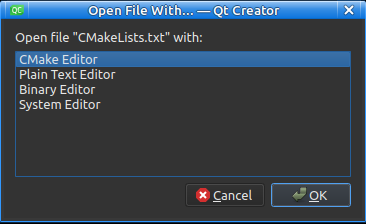
\includegraphics{open_with.png}
    \caption{Open with CMake editor.}
    \label{fig:open_with}
  \end{figure}
  
  Delete the first twelve lines, leaving
  \begin{lstlisting}
add_library(OurLib STATIC
  ourlib.cpp
  ourlib.h
)

target_link_libraries(OurLib PRIVATE Qt${QT_VERSION_MAJOR}::Widgets)

target_compile_definitions(OurLib PRIVATE OURLIB_LIBRARY)
  \end{lstlisting}

  Edit the \verb|CMakeLists.txt| file in the \verb|OurApp| directory and delete the first
  fourteen lines, so the file begins with
  \begin{lstlisting}
set(PROJECT_SOURCES
        main.cpp
        mainwindow.cpp
        mainwindow.h
        mainwindow.ui
)
  \end{lstlisting}

  We new have \verb|CMakeLists.txt| files for the \verb|OurApp| and \verb|OurLib| projects
  that contain only the information requred for each separate project. What we need now is
  a controlling top-level \verb|CMakeLists.txt| file that contains the information required
  for both projects.

  Create a new \verb|CMakeLists.txt| file. From the Qt~Creator \textbf{File} menu,
  select \textbf{New File\ldots}. In the \textbf{New File} dialog, shown in
  Figure~\ref{fig:new_txt_file}, select \textbf{General} in the left-most pane,
  and \textbf{Empty File} in the center pane, then click the \textbf{Choose\ldots}
  button.
  \begin{figure}[H]
    \centering
    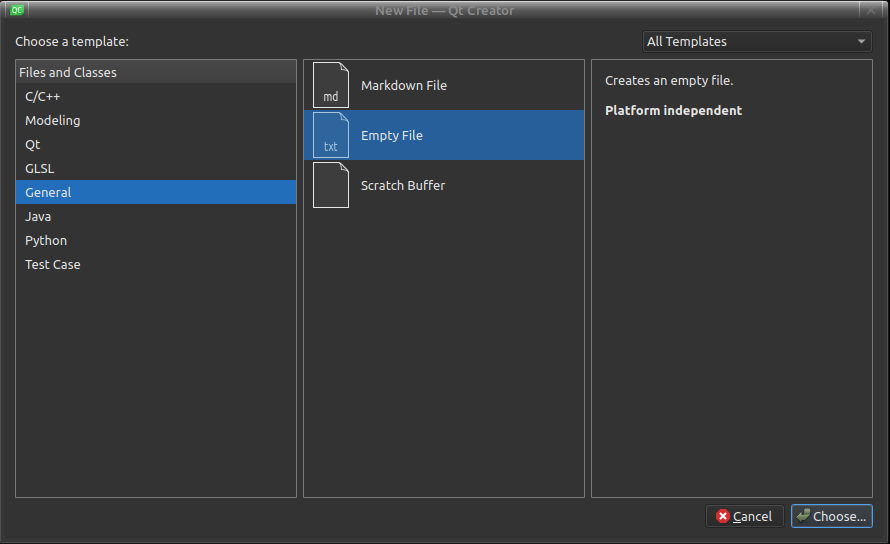
\includegraphics[width=0.7\textwidth]{new_txt_file.png}
    \caption{Create a new file.}
    \label{fig:new_txt_file}
  \end{figure}

  In the \textbf{Location} dialog (see Figure~\ref{fig:new_file_location}),
  name the file \verb|CMakeLists.txt| and place it
  in the \verb|App| directory we created earlier, one directory level up from the
  \verb|OurApp| and \verb|OurLib| directories. Click \textbf{Next}.
  \begin{figure}[H]
    \centering
    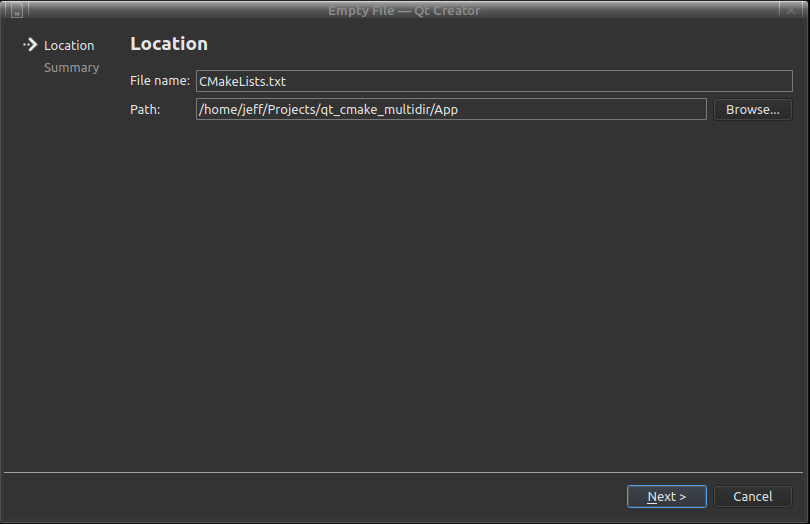
\includegraphics[width=0.7\textwidth]{new_file_location.png}
    \caption{Name and location of new file.}
    \label{fig:new_file_location}
  \end{figure}

  In the \textbf{Project Management} dialog, leave everything to the default values
  and click \textbf{Finish}.

  Add the following lines to the new \verb|CMakeLists.txt| file:
  \begin{lstlisting}
cmake_minimum_required(VERSION 3.14)

project(App VERSION 0.1 LANGUAGES CXX)

set(CMAKE_AUTOUIC ON)
set(CMAKE_AUTOMOC ON)
set(CMAKE_AUTORCC ON)
set(CMAKE_CXX_STANDARD 17)
set(CMAKE_CXX_STANDARD_REQUIRED ON)

find_package(QT NAMES Qt6 Qt5 REQUIRED COMPONENTS Widgets)
find_package(Qt${QT_VERSION_MAJOR} REQUIRED COMPONENTS Widgets)

add_subdirectory(OurLib)
add_subdirectory(OurApp)
  \end{lstlisting}

  The \verb|cmake_minimum_required| command specifies the minimum
  version of CMake required to process the project files.
  The \verb|project| command specifies the name of the project (App)
  as well as the project version number and the programming languages used.

  The \verb|set(CMAKE_AUTOUIC ON)| command specifies that \verb|CMake| will
  handle the Qt user interface compiler automatically. \verb|set(CMAKE_AUTOMOC ON)|
  specifies that \verb|CMake| will handle the Qt \verb|moc| preprocessor
  automatically, while the \verb|set(CMAKE_AUTORCC)| command tells \verb|CMake|
  to handle the Qt resource compiler automatically.

  The \verb|set(CMAKE_CXX_STANDARD 17)| and \verb|set(CMAKE_CXX_STANDARD_REQUIRED)|
  commands specify that the \Cpp\ compiler should use \Cpp17, and that this is a
  requirement.

  The two \verb|find_package| commands locate the necessary Qt libraries
  that will be required by both the \verb|OurLib| and \verb|OurApp| sub-projects.

  Finally, we need to tell \verb|CMake| that the \verb|OurLib| and \verb|OurApp| projects are sub-projects
  of the root project with the \verb|add_subdirectory(OurLib)| and \verb|add_subdirectory(OurApp)|
  commands. It is important to issue these commands in this order, with \verb|OurLib| first,
  because \verb|OurApp| depends on \verb|OurLib| and will require some information
  about the library.

  One final task remains: we must tell the \verb|OurApp| project that it needs to link
  with the library produced by the \verb|OurLib| project. Modify the \verb|CMakeLists.txt|
  file in the \verb|OurApp| directory such that the \verb|target_link_libraries| command
  includes the \verb|OurLib| library project. The updated command should now look like:
  \begin{lstlisting}
target_link_libraries(OurApp PRIVATE Qt${QT_VERSION_MAJOR}::Widgets OurLib)
  \end{lstlisting}

  Save and close all three \verb|CMakeLists.txt| files. Then from the Qt~Creator \textbf{File} menu
  select \textbf{Open File or Project\ldots} then select the new top-level \verb|CMakeLists.txt|
  file in the \verb|App| directory. Select a \textbf{Desktop} kit when prompted, then click the
  \textbf{Configure Project} button. You now have a main project with two sub-projects.
  If you expand the project tree it should look like Figure~\ref{fig:final_layout}.
  \begin{figure}[H]
    \centering
    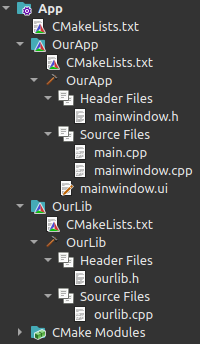
\includegraphics{final_project_layout.png}
    \caption{Layout for a main project with two sub-projects.}
    \label{fig:final_layout}
  \end{figure}

  Once you have a working top-level \verb|CMakeLists.txt| file, you may add as many
  executable or library subdirectory projects as you need. Unfortunately, Qt~Creator
  doesn't yet provide a mechanism for directly creating subdirectory projects, so
  at least for the time being you can use the \verb|CMakeLists.txt| files we created
  here as templates for new projects.
\end{document}
